% TEMPLATE for Usenix papers, specifically to meet requirements of
%  USENIX '05
% originally a template for producing IEEE-format articles using LaTeX.
%   written by Matthew Ward, CS Department, Worcester Polytechnic Institute.
% adapted by David Beazley for his excellent SWIG paper in Proceedings,
%   Tcl 96
% turned into a smartass generic template by De Clarke, with thanks to
%   both the above pioneers
% use at your own risk.  Complaints to /dev/null.
% make it two column with no page numbering, default is 10 point

% Munged by Fred Douglis <douglis@research.att.com> 10/97 to separate
% the .sty file from the LaTeX source template, so that people can
% more easily include the .sty file into an existing document.  Also
% changed to more closely follow the style guidelines as represented
% by the Word sample file. 

% Note that since 2010, USENIX does not require endnotes. If you want
% foot of page notes, don't include the endnotes package in the 
% usepackage command, below.

% This version uses the latex2e styles, not the very ancient 2.09 stuff.
\documentclass[letterpaper,twocolumn,10pt]{article}
\usepackage{usenix,epsfig}
\usepackage[small, compact]{titlesec}
\usepackage{titling}

\usepackage{tabularx}
\usepackage{graphicx}

\usepackage{verbatim} % For comment
\usepackage{xspace} % For xspace
\usepackage[pdftex,
            colorlinks,
            pdfstartview=FitH,
            linkcolor=blue,
            citecolor=black,
            urlcolor=blue,
            filecolor=black
            ]{hyperref} % For refs and urls

%\usepackage{subfig}
\usepackage[numbers,sort]{natbib}
\usepackage{paralist}
\usepackage{enumitem}
\usepackage{caption}
\usepackage{subcaption}

\graphicspath{{./figs/}}

%a few commands to highlight issues in the proposal (\TODO, \CHECK, \DummyText)
\RequirePackage{color}
\definecolor{RED}{rgb}{1,0,0}
\definecolor{BLUE}{rgb}{0,0,1}
\definecolor{White}{rgb}{1,1,1}
\providecommand{\TODO}[1]{{\protect\color{red}\noindent {\bf [TODO]} \emph{#1} {\bf [/TODO]}}}
\providecommand{\todo}[1]{{\protect\color{red}\noindent {\bf [TODO]} \emph{#1} {\bf [/TODO]}}}
\providecommand{\CHECK}[1]{{\protect\color{blue} #1 (check) }}
\providecommand{\DummyText}[1]{{\protect\color{white} #1}}
\providecommand{\tofill}[1]{{\protect\color{red} {\emph{#1}}}}

% grumble notes
\usepackage{ifthen}
\newboolean{publicversion}
\setboolean{publicversion}{true}
\ifthenelse{\boolean{publicversion}}{
  \newcommand{\grumbler}[3]{}
}{
  \newcommand{\grumbler}[3]{\textcolor{#3}{\bf #1: #2}}
}

\newcommand{\vc}[1]{\grumbler{Vijay}{#1}{red}}
\newcommand{\ak}[1]{\grumbler{Aasheesh}{#1}{blue}}
\newcommand{\rk}[1]{\grumbler{Rohan}{#1}{green}}

%\providecommand{\vc}[1]{{\protect\color{red} \textbf{Vijay:} #1}}
%\providecommand{\ak}[1]{{\protect\color{blue} \textbf{Aasheesh:} #1}}
%\providecommand{\rk}[1]{{\protect\color{green} \textbf{Rohan:} #1}}

\newcommand{\ra}[1]{\renewcommand{\arraystretch}{#1}}

\newcommand{\mycaption}[2]{\caption{\textbf{#1}. \textit{#2}}}
\newcommand{\sref}[1]{\S\ref{#1}}
\newcommand{\vheading}[1]{\vspace{0.05in}\noindent\textbf{#1}}
\newcommand{\viheading}[1]{\vspace{0.05in}\noindent\emph{#1}}
\newcommand{\fsync}{\texttt{fsync()}\xspace}
\newcommand{\etal}{\textit{et al.}\xspace}
\newcommand{\ie}{\textit{i.e.,}\xspace}
\newcommand{\eg}{\textit{e.g.,}\xspace}
\newcommand{\etc}{\textit{etc.}\xspace}
\newcommand*{\affaddr}[1]{#1} % No op here. Customize it for different styles.
\newcommand*{\affmark}[1][*]{\textsuperscript{#1}}
\newcommand*{\email}[1]{\texttt{#1}}
\newcommand{\myx}{$\times$\xspace}
\newcommand{\vtt}[1]{\texttt{#1}\xspace}
\newcommand{\mytitle}{CSR: Small: Collaborative: Solving the Dirty-Data Tracking Problem in
  Persistent Memory Systems}
\newcommand{\mye}{$\epsilon$\xspace}
\newcommand{\lget}{\texttt{get()}\xspace}
\newcommand{\lput}{\texttt{put()}\xspace}
\newcommand{\lrq}{\texttt{range\_query}\xspace}
\newcommand{\lseek}{\texttt{seek()}\xspace}
\newcommand{\lnext}{\texttt{next()}\xspace}
\newcommand{\msync}{\texttt{msync()}\xspace}
\newcommand{\syswrite}{\texttt{write()}\xspace}
\newcommand{\sysread}{\texttt{read()}\xspace}
\newcommand{\movnti}{\texttt{movnti}\xspace}
\newcommand{\memcpy}{\texttt{memcpy()}\xspace}
\newcommand{\mmap}{\texttt{mmap()}\xspace}
\newcommand{\mmaped}{\texttt{mmap}-ed\xspace}
\newcommand{\sync}{\texttt{sync}\xspace}
\newcommand{\xtimes}{$\times$\xspace}
\newcommand{\mapprivate}{\texttt{MAP\_PRIVATE}\xspace}
\newcommand{\mapshared}{\texttt{MAP\_SHARED}\xspace}
\newcommand{\seq}{\texttt{seq}\xspace}
\newcommand{\rand}{\texttt{rand}\xspace}
\newcommand{\stride}[1]{\texttt{stride-{#1}}\xspace}
\newcommand{\llr}[1]{\texttt{linked-list-{#1}}\xspace}
 % For macros

\setlength{\droptitle}{-4em}
%\posttitle{\par\end{center}}

\begin{document}

%don't want date printed
\date{}

%make title bold and 14 pt font (Latex default is non-bold, 16 pt)
\title{\Large \bf StrataSGX: Securing Strata with Intel SGX}

\author{
{\rm William Lin}
%University of Texas at Austin\\
\qquad
{\rm Kishan Patel}
\qquad
{\rm Noah Thornton}
\qquad
{\rm Tiffany Yang}
    \vspace{2pt}\\
%University of Texas at Austin and VMware Research
\emph{The University of Texas at Austin}
%\qquad
} % end author
%\fi

\maketitle

\section{Abstract}

The initial goal of the project was to reduce the amount of metadata leaked by
Strata, a state-of-the-art cross-media file system, by utilizing Intel's
Software Guard Extensions (SGX). However, we quickly realized our knowledge of
both the current literature on systems security and of the details of Intel's
SGX was limited. In this paper, we detail our findings from the relevant
papers and present existing applications of SGX.  Then, we present our
modification to Strata: the duplication of the kernel-level digest process as
a separate user-level thread. This change potentially reduces the metadata exposed, 
protecting against a malicious privileged software stack. We also discuss the
usefulness and practicality of running \verb|libfs| inside of hardware
enclaves.


\section{Introduction}

Datacenters are at the root of many popular services such as Netflix, Facebook,
and Google. Due to economies of scale, it is often cheaper and more
efficient for companies to rent computing resources from services such as
Amazon AWS, Microsoft Azure, or Google Cloud. Services offered have greatly
diversified in recent years from the traditional virtual machine model. New
services provided to customers include bare-metal instances, containers, and more 
recently, serverless models. With these new models, datacenter providers
have total control over the stack used by the consumers.  Consequently, these
providers have the ability to manipulate the hardware, the operating system,
and the management software.  Therefore, by running applications on top of these
datacenter services, users place enormous trust onto these providers to
maintain the security and integrity of their services. It is upon the
customer to try and secure their secrets against the cloud provider and
independent attackers.
%but also to secure their services against independent attackers ranging from
%other customers to malicious system administrators. 

%They are also used for computation on private user data and
%sensitive secrets. play a significant role in society. Since they host 

\section{Background}
\subsection{SGX}
SGX is the set of new hardware instructions that were introduced by Intel in 2015 to
support the secure execution of a user process inside of an \emph{enclave}. An
application utilizing SGX is divided into a secure and an unsecured portion.
The secured component of the process is placed in an enclave that protects a
portion of the virtual address space via hardware encryption. This protection 
prevents higher level attackers, even hypervisors and the OS kernel, from accessing
or modifying pages store in the enclave memory.


The pages that will be protected by an enclave are specified by the application
developer and kept in the Enclave Page Cache (EPC). Before each insertion into
the TLB after a TLB miss, the linear address is checked against the EPC to
ensure that only code executing within the enclave can access a protected page.
This check is performed in hardware by the Intel CPU die. Consequently, the
application does not need to trust the entire OS and hypervisor stack, only the
CPU package.

Applications executing within an
enclave can write and read freely to other valid parts of the address space;
however, SGX hardware does not ensure their integrity, so the responsibility of
verifying and securing those memory accesses falls to the enclave code. 

% I dont really think this is relivant
%\todo{ECREATE, EADD}


\subsection{SGX Limitations}
\subsubsection{Enclave Page Cache Size}
The size of the enclave page cache is limited to 128 MB. SGX will swap
pages in and out of enclave memory when necessary, but this activity is costly.
The entire outgoing page must be encrypted before being written out to DRAM,
and then the page coming in must be decrypted and verified. 

SGX protects enclave memory by encrypting the page at the granularity of a
cache line. When a cache miss occurs, the memory encryption engine must first
decrypt the cache line before inserting it into the L3 cache. The SCONE~\cite{arnautov_scone:_2016}
paper contains a detailed analysis of this limitation. It is orders of
magnitude slower for random accesses versus sequential ones. Sequential
accesses benefit from the CPU prefetching mechanism, which helps to amortize
the cost of enclave cache misses. 

%% maybe state that we will limit our discussion of possible attacks to filesys?

\subsubsection{Security Vulnerabilities}
Along with these performance challenges, Intel SGX is still vulnerable to a
range of side-channel attacks. Three common side-channel attacks are system
call snooping, page fault attacks, and cache-channel attacks; the
responsibility of defending against these types of attacks is delegated to the
application developer.

% Maybe write about how the kernel is hard to protect from bc it has so much "authority"

SGX enclaves are designed to run with user-level privileges, so control must 
leave the enclave for an application to access system resources. 
Calls outside of the enclave can be made using \verb|OCalls|. 
When a system call is forwarded to the kernel using an \verb|OCall|, the 
untrusted kernel gains access to the function arguments and its return value. 
When file system calls are made, the file being accessed and/or the 
exact offset of the file read or write can be tracked by the kernel. Even 
encrypted files do not offer significant improvements to security because 
their encryption schemes are likely on the block level. This convention allows 
a single block to be accessed and decrypted instead of requiring the decryption 
of the entire file. Although an attacker may not be able to read the data 
directly, the kernel has full knowledge of the order in which blocks are 
accessed. Savvy attackers can gather significant insights from observing these 
file access patterns. 

%This exposure presents two types of security risks. 

%move this to iago attacks?
%Since the return value originates from the untrusted domain, it is 
%possible that the \verb|OCall| function was never performed.
%Suppose that an enclave requests to write data to a block device. 
%A compromised system could return a value indicating that an enclave's request 
%was successfully executed when in reality the file-write was dropped. 

%% TODO: write more in detail here


Another way a malicious kernel can learn about a program executing in an
enclave is through its memory access patterns.  The kernel can force page
faults by evicting the application's pages or changing page table permissions
to mark them non-accessible, allowing it to see which pages the program is
accessing.  Repeated faults on the same memory address can show the attacker
the location of the application's in-memory file buffer.  If the attacker can
contextualize one address in the layout of the file, then observing the
location of other page faults relative to that address gives them the ability
to calculate the offset of each file access or to learn the sizes of the data
structures within the file. SGX slightly mitigates the information leaked to
the kernel by clearing the page offset before context switching, which limits
the level of detail to the system's page size.

Most memory reads or writes are placed in the cache. Thus, the cache provides
meaningful insight into the memory activity on the computer.  In an inclusive
cache hierarchy, blocks that are present in a higher-level cache are also
present in the lower-level cache. Conversely, data that is removed from the L3
cache, which is shared among all users, must also be removed from higher-level
caches. An adversarial system can exploit this design to learn about the
protected application. In a \emph{prime and probe} attack, the attacker first
primes a cache set by accessing memory locations at known addresses to place
those addresses into the cache. Next, they wait for the victim application to
execute. Finally, they time how long it takes to access the original known
addresses. A relatively slow re-access indicates a cache miss, informing the
attacker that the victim used memory that maps to the same cache set. Using
this method, the attacker gains information about memory accesses that can be
used to learn about files in a similar fashion to the page-fault attacks
discussed above.

For all three of these side-channel attacks, file-encryption fails to provide
sufficient protection from an untrusted kernel.  In a syscall snooping attack,
if an attacker already knows the layout of a file, they can use the offset of a
file read to determine the data being read.  For certain types of files,
tracking repeated access patterns is sufficient to deduce how that file is
arranged.


\section{Security and Related Works}
\subsection{Iago Attacks}
In 2013, Checkoway and Shacham introduced a new class of attacks called
\emph{Iago Attacks}. These attacks are a type of syscall attack used against 
systems running on untrusted operating systems (Iago~\cite{checkoway_iago_2013}). 
This paper showed that, despite existing protection mechanisms 
(Overshadow~\cite{chen_overshadow:_2008}) that prevent the kernel from directly 
reading or writing protected application memory, similar to the protection 
provided by SGX, Iago Attacks can still cause the application to act against its 
own interest in the best case, and undertake arbitrary code execution in the 
worst. Checkoway and Shacham's paper details how a carefully chosen sequence of
integer return values to Linux system calls can be returned to the application
by a malicious kernel to compromise an application.


It is not enough to merely prevent privileged software from accessing or
modifying protected application memory. The results of system calls to the
potentially malicious kernel also have to be verified to prevent compromising
security. Linux's system call API was not originally designed to be an
untrusted RPC interface, making it a troublesome interface to secure. Additionally, 
the size of the interface has been steadily growing, further increasing the 
attack surface against applications.

\subsubsection{Overshadow/SGX}
The Overshadow~\cite{chen_overshadow:_2008} system mentioned above was used in
a paper as a model for the preexisting protection around a process under
attack. The Overshadow hypervisor has higher privileges, allowing it to both
protect the process and allow it to run trusted code. Unlike XOMOS and Flicker,
which provide these capabilities through trusted hardware, Overshadow relies on
running as a hypervisor. Intel saw the need for hardware to provide a trusted
computation base, and thus SGX provides similar security guarantees to systems
like Overshadow. Using trusted hardware as the protection mechanism has obvious
benefits, such as a reduced trust domain and performance improvements to
systems such as Overshadow. However, it still has many vulnerabilities such as
Iago attacks.

%\todo{if we need to fill more space we can include examples of attacks (use of
%getpid)}

\subsection{Library OS}
To protect against Iago attacks, system call parameters must be encrypted, and 
their return values sanitized. SGX does not provide these functions, so it 
cannot protect against Iago attacks.  To maintain security, SGX prohibits system
calls from being made inside of an enclave. While this allows the results of 
system calls to always be sanitized by \emph{shielding code} within the enclave 
before use, it prevents applications from running on SGX unmodified.

For both portability and as an abstraction layer to facilitate quick
development, a library OS is typically loaded into the enclave and
use by the application. The library OS will then interact and perform
operations on behalf of the enclave process through a well-defined interface to
the host OS. There is a range of literature on what the trade-off between the
size of this interface with the host and the size of the trusted
computing base of the library OS should be. A larger interface has a larger
potential to be exploited by attackers, but it is also able to keep the library 
OS smaller, as more functionalities can be derived from the richer interface.
A smaller interface gives attackers a reduced attack surface but comes at the
cost of bloating the size of the library OS, and thus the TCB, in an effort to
provide those lost functionalities directly in the user space.


\subsubsection{Graphene-SGX}
Graphene-SGX~\cite{tsai_graphene-sgx:_2017} is a port of the
Graphene~\cite{tsai_cooperation_2014} library OS to SGX. It is designed to
allow general applications to be quickly adapted for the limitations imposed by
SGX.  The authors of Graphene-SGX found that the large TCB size attributed to a
library OS can be mostly eliminated by either compiling out unused
functionalities, as in a unikernel~\cite{madhavapeddy_unikernels:_2013}, or by further partitioning an application
into multiple enclaves with fewer syscall requirements. Due to these findings,
they decided to keep the interface to the host OS minimal and let application
developers optimize code and reduce TCB as needed after bringing up the
application on SGX.

In addition to providing the SGX application with the classic Graphene library
OS, Graphene-SGX also includes an SGX-specific platform adaptation layer (PAL).
The PAL implements 36 functions of the host ABI against which the library OS is
programmed. PAL then interacts with the Host OS through an even smaller set of
28 interfaces. The smaller interface to the Host OS enables Graphene-SGX to
also act as the \emph{shielding code} that verifies the untrusted kernel's
behavior. The extra layer of indirection allowed the authors to carefully
define the semantics of the ABI, which enabled meaningful run-time checks to
validate responses from the kernel.

%\todo{maybe put a list of examples here?}

\subsubsection{SCONE}
SCONE provides a secure way to execute Linux containers utilizing Intel SGX.
This option allows for the use of Docker with slight modifications to run
containers in an enclave. Docker is already heavily deployed in the datacenter
world, so allowing the same tooling to be used to run and manage unmodified
Linux applications securely in an untrusted cloud is desirable.

This mechanism is implemented with a few things in mind. Similar to the
findings in Graphene-SGX, the authors of SCONE aimed to minimize the size of
the TCB in combination with a library to provide a secure system call interface
to the containers. Instead of using a full-fledged library OS such as Graphene
inside the enclave, SCONE links in musl libc (88k LOC), a much smaller libc
implementation than glibc (1195k LOC) to the enclave. Due to this choice,
applications running on SCONE are only given the C Library interface to work
with versus the full range of syscalls provided by a library OS. Notably, SCONE
does not support system calls such as \verb|fork|, \verb|exec|, and
\verb|clone|. The SCONE authors make the argument that containers typically
execute network services such as
Memecached~\cite{fitzpatrick_distributed_2004},
Apache~\cite{noauthor_welcome!_nodate}, NGINX~\cite{reese_nginx:_2008}, and
Redis~\cite{noauthor_redis_nodate}, which require only a limited interface for
communication with the outside. 

%\todo{talk about is this worth it}



%This library runs asynchronously, to minimize
%exits from the actual enclave. It provides the secure interface using what they
%call shields. These shields sanitize and communicate securely.

\subsection{Data Oblivious}
Datacenter applications are composed of many inter-communicating components.
Whether this communication is done through messages, shared memory, or
procedure calls, it all involves the transfer of data and metadata to another
component or system. At the boundary of these interfaces used for
communication, determined attackers can monitor the traffic pattern of these
channels and glean secrets, despite not being able to decipher the encrypted
data payload.  For example, a malicious kernel could record the frequency,
size, and location of \verb|read| system calls to infer results of database
queries.

The Obliviate~\cite{noauthor_obliviate:_nodate} paper contains a case study of
an attack of this type against a SQLite database storing privacy-sensitive
information indicating whether a person has a history of heart diseases in
his/her family. By analyzing the patterns of system calls the Obliviate authors
were able to pinpoint the exact row and column of the SQLite database accessed.

Beauty and the Burst~\cite{schuster_beauty_2017} also details how a
convolutional neural network can be used to remotely identify encrypted video
streams by classifying the burst patterns of the MPEG-DASH streaming video
standard common to many video hosting sites such as Youtube and Vimeo.
Specifically, the authors were able to identify the exact video streamed to the
target machine by observing network traffic patterns through a Javascript ad
confined to a web browser on a nearby machine.

\subsubsection{Oblivious RAM}
Oblivious RAM (ORAM) provides obfuscated access to encrypted memory that
prevents the data access patterns from leaking any important information about
the underlying data. The key idea behind ORAM is to obfuscate access by
shuffling and re-encrypting blocks of memory after each access so that an
attacker cannot determine which memory region is being accessed, even with
repeated runs of the program. The ORAM protocol allows data blocks stored
on an untrusted machine to be accessed in a uniform pattern (to an external
observer) regardless of the actual workload, e.g., repeatedly reading the same
data block.

\subsubsection{Obliviate}
Obliviate is an in-memory SGX file system designed to protect SGX application
from insidious side-channel attacks such as page fault, cache-based, and
syscall snooping attacks. The Path ORAM protocol is used to obscure the access
patterns of each application to DRAM. Path ORAM is an optimization of ORAM
that uses a complete binary tree to store encrypted blocks of memory on the
untrusted DRAM outside of the SGX enclave. Each node in the binary tree holds
multiple data blocks, and each data block is either a dummy block or a block that
holds real data. The number of real blocks in a PATH ORAM tree is always equal
to the number of leaf nodes in the binary tree, and the blocks are randomly
distributed throughout the tree. The remaining blocks are filled with dummy
data. Obliviate maintains a \emph{Position Map} inside the enclave that
specifies a path to a unique leaf node for each real data block in the tree.
The real data block is found somewhere on the path to the leaf node, and
regardless of where the real data block is located on the path, the tree is
always traversed to the leaf in order to obfuscate the actual location.  As
real data blocks are encountered, they are decrypted and copied into a
\emph{Stash} region inside the enclave, which caches a number of real data
blocks.

While this does allow Obliviate to protect against all side channels, it comes
at the cost of almost 200x slowdowns compared to standard file systems.


\subsection{Ryoan}
Ryoan~\cite{hunt_ryoan:_2016} is a model to enable secure computation on an untrusted cloud,
focusing on request oriented computation. As with other related works, Intel
SGX is the key that makes this possible. Ryoan utilizes a sandbox similar to a
library OS, Google Native Client (NaCl)~\cite{yee_native_2009}. NaCl is used to verify that the
application code cannot escape the sandbox and intercept system calls.  Thus,
viewing sensitive data or code is obscured in memory by SGX, and system calls
are redirected to trusted code provided by Ryoan. This design allows for
privacy and security during execution, but communication still provides a large
attack surface.  In order to address this, there is only one phase in which
input can be read in from outside of the sandbox and one phase for output from
the sandbox. Data is encrypted during these communications and sent in regular
intervals with a constant size.  This is done by padding small messages with
garbage data or splitting larger messages into fixed-size chunks. By doing
this, the data is secure from service provider snooping, and the metadata
provides no useful patterns.

One thing of note is the lack of external file access during computation.
Ryoan provides a virtual, in-memory file system to avoid the security
vulnerabilities associated with file systems. Intel SGX thus obscures all file
contents, and metadata is not leaked through file system accesses. The authors
state that if something like a database is larger than memory, it can be split
into multiple sandboxes due to their composability. A point of interest is that
the authors considered using the ORAM protocol but decided that it would be too
much of a performance hit.


%Maybe talk about how it is composable 
%also talk about how files are not considered they are all in virtual filesystems

%\end{description}

\section{Design}

The design goal for StrataSGX is to minimize the amount of metadata sent to the
kernel. Any file system has a substantial surface area to defend. Our
%There is a lot of surface area to defend in a secure file system; Our
method of shielding metadata specifically targets syscall snooping. We focus on
this type of attack because Strata's functionality relies heavily on the
kernel. Furthermore, of the various attacks we encountered in the literature,
we determined that syscall snooping is the most easily exploited in Strata.
Therefore, to reduce the degree of access a potentially malicious kernel could
have, we shift as much responsibility from KernelFS to LibFS as possible.

\subsection{Threat Model}

StrataSGX follows a typical threat model for SGX applications. All
hardware components outside of the CPU are untrusted, and they can coordinate with
software to attack the application. Traditionally trusted components such
as the OS and hypervisors are now powerful attackers with \emph{superuser}
privileges. Other applications executing on the same host, including unrelated
enclaves and user-space components of the same application that exist outside of
its enclave's protection are also untrusted. We only trust Intel's CPU package,
the implementation of SGX SDK, the enclave code, %including the libc or library OS, 
the unmodified application, and its supporting libraries.

Untrusted components can collude to attack the enclave and learn application
secrets. As previously discussed, these attacks can involve syscall snooping,
page-fault attacks, and cache-based attacks. Unlike our paper, many papers
using SGX do not protect against these attacks in their threat models; however,
their omission of side-channel attacks does not indicate that side-channels
irrelevant. Only that they are difficult to secure against.  SGX is
specifically designed to protect against privileged hypervisors and kernels
that fall outside of the domain of trust.  It is entirely feasible for
attackers to use side-channel vulnerabilities to gain access to application
secrets.

\section{Implementation}

%The implementation covered below describes how we account for the threat model
%presented in the previous section.  
To reduce the amount of user-data exposed
to the kernel while attempting to retain Strata's performance benefits, %part
of the KernelFS digest, we introduced user log coalescing into LibFS.  This
functionality was implemented directly on top of Strata. 
Unlike Strata, where the entirety of the user log is accessible
by the kernel, the user log in StrataSGX is separated into two parts.
We reserved 30\% of the log per process to be placed outside of SGX for the kernel 
to be able to read from. LibFS performs all of its writes to the other 70\% of the 
log, which resides within the enclave.
Whenever the SGX log reaches a certain capacity, a coalesce request is made to a 
thread that coalesces the transactions in user mode and then copies it over to the 
non-SGX log for the kernel to digest. 
Ideally, the coalesced data should be encrypted using a block-cipher before being 
written to the shared log portion, which we leave as future work. Similarly, since
the kernel must have unencrypted metadata to write the encrypted data to the
file system, future implementations should intersperse chaff within the shared log 
to introduce noise to the file system accesses observed by the system. 
After coalescing, a synchronous request to the kernel is made to digest the 
data from the non-SGX log. 

%We considered several aspects in designing StrataSGX.
When implementing StrataSGX, we did not have access to an SGX-enabled machine.
Here we will discuss the predicted impacts of our design choices on
StrataSGX's performance. 
%%% AHHHHH THIS IS SHIT (all of this sorry)
The relatively small capacity of the non-SGX log means that more than one KernFS 
digest may be required to free up space if the coalesce request from the SGX log is 
too big. Reserving a larger percentage for the non-SGX log mitigates this issue, 
but also results in more frequent LibFS coalesce requests from the SGX log. 

Like the original KernelFS digest, StrataSGX LibFS coalescence prunes redundant 
operations from the user-level log. By coalescing the log in the user space
before requesting kernel digest, certain details about the protected
application's file system operations can be obfuscated from the kernel.
Moreover, in the context of a protected file system, coalescence would reduce the
quantity of data that the application must encrypt before writing to the shared
portion of the log, thereby improving the performance of the system.


\section{Evaluation} \label{eval}

%\subsection{\large 5.1 Measurement Techniques}
In this section, we evaluate performance metrics for StrataSGX. %The performance
%will be compared to the performance of Strata. 
As indicated in Figure \ref{fig:microbench}, StrataSGX achieves about %slightly more than  
half of the throughput that Strata does for file writes. This discrepancy can be 
attributed to the overhead of copying the SGX-portion of the log to the non-SGX 
portion for kernel digest. Although the duplication of data results in a 
significant performance hit to StrataSGX, the process of coalescing logs within 
LibFS minimizes the amount of data that must be copied to the non-SGX log. 
The effects of this optimization are observable in the cases where Strata averages 
less than double the throughput of StrataSGX.

While performance is important, the 
goal of this project was to minimize metadata leakage to the malicious kernel. The 
process of coalescing the SGX log in user mode also facilitates the process of 
obscuring the data the kernel sees. After coalescing logs, file reads and
writes can be performed using the ORAM protocol to obscure the actual block
being accessed. The projected effects of implementing the ORAM functionality in
StrataSGX indicate write throughputs that are an order of magnitude worse
(200x) than both Strata and StrataSGX, shown in Figure \ref{fig:microbench}.

\begin{minipage}{\linewidth}
\centering
    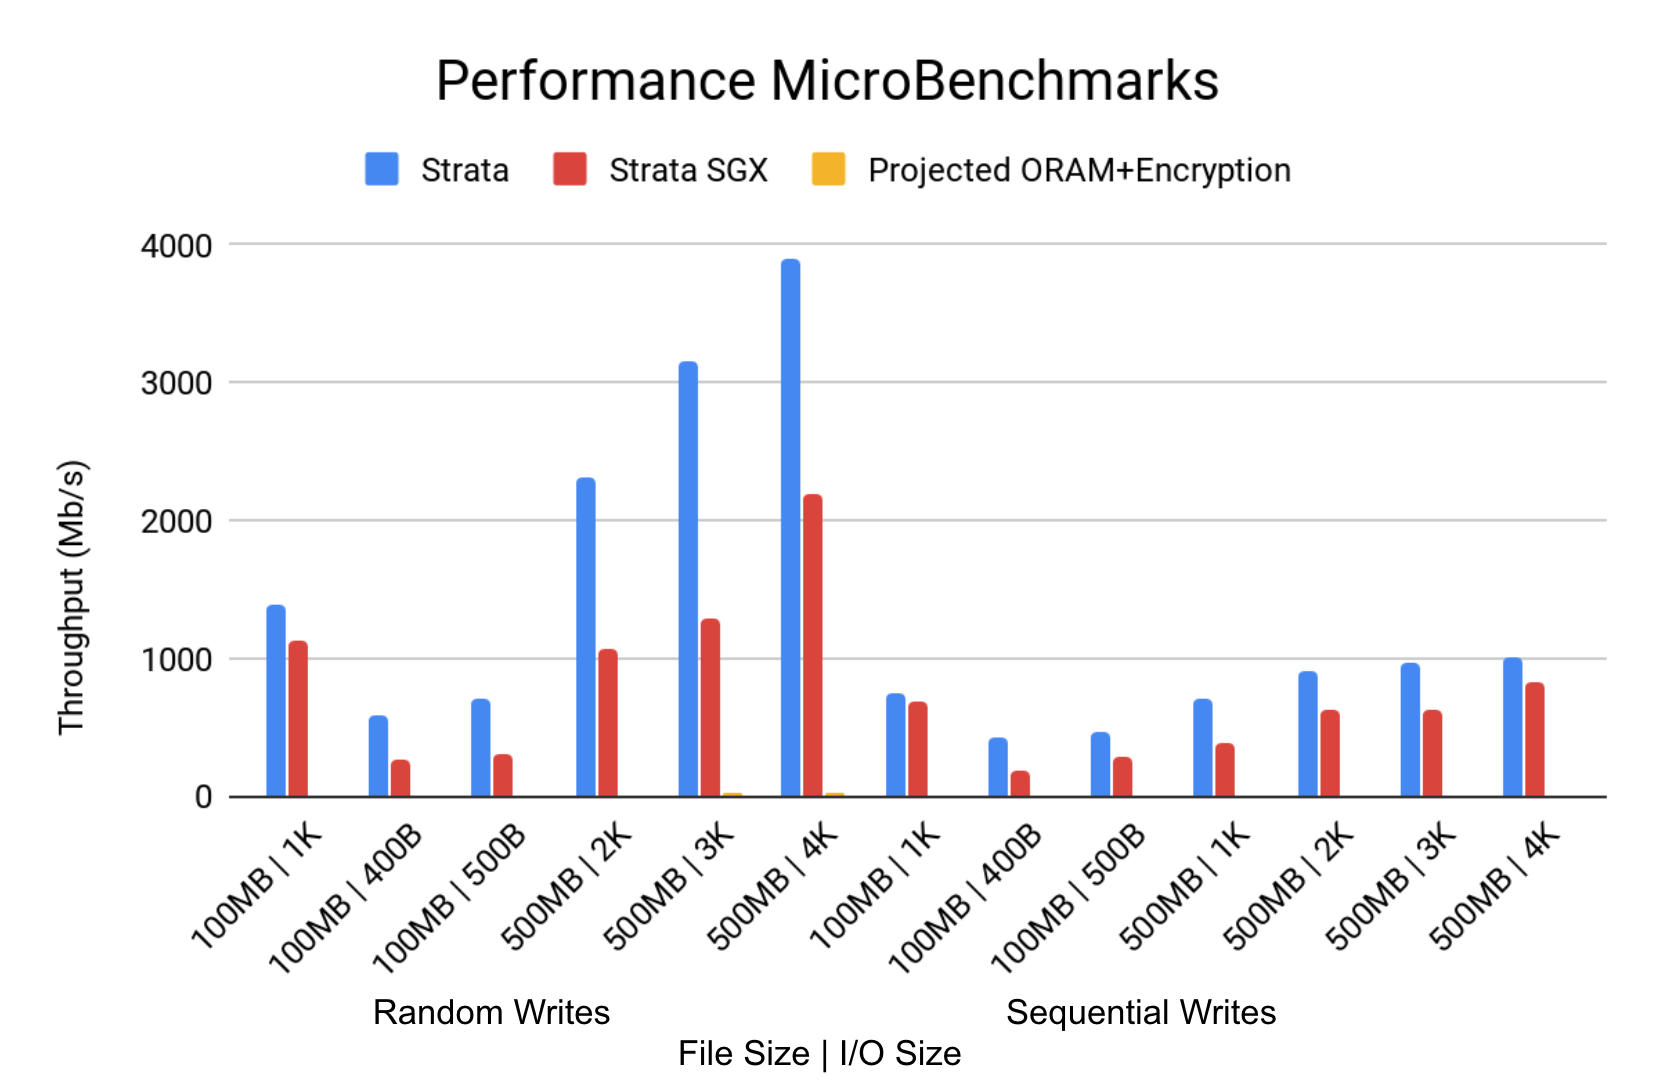
\includegraphics[width=\textwidth]{performance.png}
      \captionof{figure}{Write throughput under filesys models}
      \label{fig:microbench}
\end{minipage}
\\

%\begin{center}
    %\begin{table}
    %\begin{tabularx}{.89\columnwidth}{ | l | c | }
        %\hline
            %& \emph{Configuration} \\ \hline \hline
            %Processor & Intel i7-8700K @ 3.70GHz \\ \hline
            %CPU Cores & 6 \\ \hline
            %L1 & 32 KB i + 32 KB d per core\\ \hline
            %L2 & 256 KB \\ \hline
            %L3 & 12288 KB \\ \hline
            %Memory & 24 GB \\ \hline
            %%GPU & 1 X NVIDIA Quadro K420 \\ \hline
            %%GPU cores & 192 \\ \hline
            %%GPU Memory & 1 GB DDR3 \\ \hline
            %OS & Ubuntu 18.04.4 LTS \\ \hline
            %SSD & Samsung 860 EVO SATA 6Gb/s\\
            %%Network & 1 Gigabit Ethernet \\
        %\hline
    %\end{tabularx}
        %\caption{Machine spec.}
        %\label{server spec}
    %\end{table}
%\end{center}



\section{Conclusion}

Many of the features that allow Strata to provide excellent performance make it
poorly suited to provide security against a compromised system.  Reducing
Strata's reliance on the kernel resulted in a significant decrease in its
performance. Furthermore, this implementation is still heavily susceptible to
side- channel attacks, but it is likely that modifications to further reduce
Strata's vulnerability to those attacks would be too costly to its operation to
justify.  The current implementation of StrataSGX forgoes encryption between
the SGX and non- SGX portions of the log, but under the projected benchmarks,
the detrimental impact on performance makes the necessary encryption untenable.
Likewise, introducing chaff using ORAM to obscure the metadata seen by the
kernel is left to future work.  This study has shown that Strata works
exceptionally well in a trusted system, but its design is fundamentally unfit
to provide security in this context.

%
%\section{Future Work}
%
%\todo{Talk about how we did not use an enclave??}

\newpage
\pagebreak

{\footnotesize \bibliographystyle{acm}
\bibliography{all}}

\end{document}







